\documentclass[10pt]{article}
\usepackage[polish]{babel}
\usepackage[utf8]{inputenc}
\usepackage[T1]{fontenc}
\usepackage{graphicx}
\usepackage[export]{adjustbox}
\graphicspath{ {./images/} }
\usepackage{amsmath}
\usepackage{amsfonts}
\usepackage{amssymb}
\usepackage[version=4]{mhchem}
\usepackage{stmaryrd}

\title{GIMNAZJUM }

\author{}
\date{}


\begin{document}
\maketitle
\begin{enumerate}
  \item W grupie siedmiu chłopców każdy ma co najmniej trzech braci. Udowodnij, że jest to grupa siedmiu braci.
  \item Na brzegu jeziora w kształcie koła znajdują się cztery przystanie: K, L, P, Q. Z przystani K wypływa kajak kierując się do przystani Q, a z przystani L w tym samym momencie wypływa łódka kierując się do przystani P. Wiadomo, że gdyby zachowując swe prędkości kajak popłynął w kierunku przystani P, a łódka w kierunku przystani Q, to doszłoby do zderzenia. Udowodnij, że kajak i łódka dobiją do\\
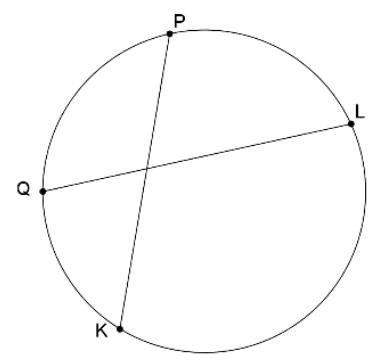
\includegraphics[max width=\textwidth, center]{2024_11_21_4102729fe0ded42594c6g-1}\\
celu w tym samym czasie.
  \item Znajdź wszystkie trójki liczb pierwszych spełniających równanie:
\end{enumerate}

\[
a \cdot b \cdot c=5(a+b+c)
\]

\section*{LICEUM}
\begin{enumerate}
  \item Jak czworokąt wypukły ABCD podzielić na dwie części o równych polach prostą przechodzącą przez wierzchołek A?
  \item Wyznacz taką największą liczbę naturalną \(k\), aby dla każdej liczby naturalnej nieparzystej \(n\) liczba \(n^{6}-n^{4}-n^{2}+1\) była podzielna przez \(2^{k}\)
  \item Wykaż, że w każdym równoległoboku suma kwadratów długości przekątnych równa jest sumie kwadratów długości wszystkich jego boków.
\end{enumerate}

\end{document}